\documentclass{JNUexp}
\courseName{Linux 环境程序设计}
\expName{实验 4 shell 编程}
\expDate{2017.11.09}
\className{计科1404}
\studentName{阎覃}
\studentId{1030414414}

\graphicspath{ {images/} }

\usepackage[hidelinks]{hyperref}
\begin{document} 

\section{实验目的}
\begin{itemize}
    \item 了解shell的作用和主要分类;
    \item 掌握bash的建立和执行方式;
    \item 掌握bash的基本语法;
    \item 学会编写shell脚本。
\end{itemize}

\section{实验内容}
\begin{itemize}
    \item shell 脚本的建立和执行
    \item shell 变量和位置参数;
    \item 一般控制结构。
\end{itemize}
\section{实验步骤及运行情况}
%%%%%%%%%%%%%%%%%%%%%%%%%%%%%%%%%%%%%%%%%%%%%%%%%%%%%%%%%
%   1
%%%%%%%%%%%%%%%%%%%%%%%%%%%%%%%%%%%%%%%%%%%%%%%%%%%%%%%%%
\begin{problem}
    利用 vi 建立一个脚本文件,其中包括 date、cal、pwd、ls 等常用命令。然后以不同方式执行该脚本.
\end{problem}

\begin{answer}
    首先进入vim创建名为test1.sh的脚本
    \begin{lstlisting}[language=sh]
vim ./test1.sh
    \end{lstlisting}
    之后输入以下脚本
    \lstinputlisting[language=sh,title=test1.sh]{../test1.sh}
    \subparagraph{方法1} 直接执行脚本
        \begin{lstlisting}[language=sh]
chmod +x ./test1.sh  #使脚本具有执行权限
./test1.sh  #执行脚本
        \end{lstlisting}
    \subparagraph{方法2} 作为解释器参数
        \begin{lstlisting}[language=sh]
/bin/sh test1.sh
        \end{lstlisting}
\end{answer}

\begin{image}
    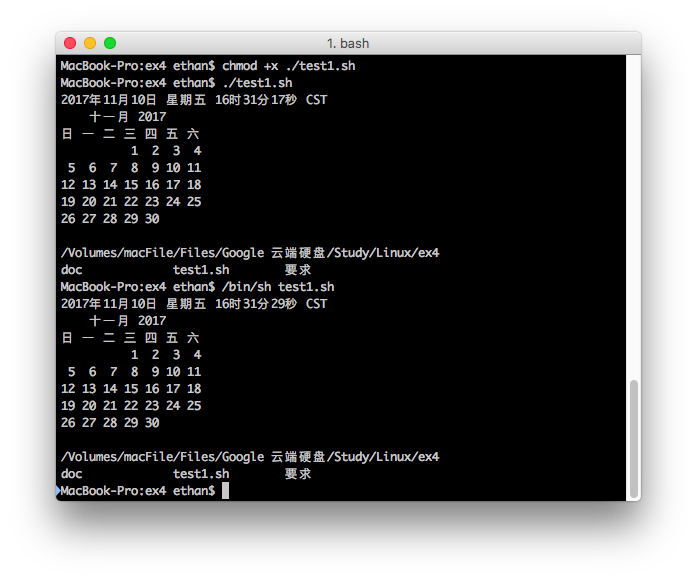
\includegraphics[width=0.7\textwidth]{1}
    \caption{shell脚本执行常用命令}
\end{image}



%%%%%%%%%%%%%%%%%%%%%%%%%%%%%%%%%%%%%%%%%%%%%%%%%%%%%%%%%
%   2
%%%%%%%%%%%%%%%%%%%%%%%%%%%%%%%%%%%%%%%%%%%%%%%%%%%%%%%%%
\begin{problem}
    利用变量赋值方法,将字符串\lstinline{DOS file c:>\student\*}显示出来.
\end{problem}

\begin{answer}
    新建test2.sh 输入以下脚本
    \lstinputlisting[language=sh,title=test2.sh]{../test2.sh}    
\end{answer}

\begin{image}
    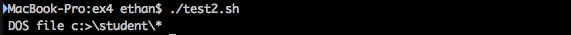
\includegraphics[width=0.7\textwidth]{2}
    \caption{shell脚本显示特殊字符}
\end{image}

%%%%%%%%%%%%%%%%%%%%%%%%%%%%%%%%%%%%%%%%%%%%%%%%%%%%%%%%%
%   3
%%%%%%%%%%%%%%%%%%%%%%%%%%%%%%%%%%%%%%%%%%%%%%%%%%%%%%%%%
\begin{problem}
分析下列 shell 脚本的功能:

\lstinputlisting[language=sh]{../test3.sh}

\end{problem}

\begin{answer}
    \lstinline{$#}代表的是传递给脚本参数个数; \\
    \lstinline{\$$count} 转义后即
    \lstinline{$2},
    \lstinline{$1},\ldots,表示命令名后面的参数;\\
    \lstinline{count=`expr $count - 1`},将变量count自减1。\\
    最后的cmd可以得到如下形式:
    \lstinline{echo $2 $1},即将所有参输出。
\end{answer}
%%%%%%%%%%%%%%%%%%%%%%%%%%%%%%%%%%%%%%%%%%%%%%%%%%%%%%%%%
%   4
%%%%%%%%%%%%%%%%%%%%%%%%%%%%%%%%%%%%%%%%%%%%%%%%%%%%%%%%%

\begin{problem}
编写一个 shell 脚本,它把第二个位置参数及其以后的各个参数指定的文件复制到第一个位置参数指定的目录中.
\end{problem}

\begin{answer}
    \lstinputlisting[language=sh,title=test4.sh]{../test4.sh}
\end{answer}

\begin{image}
    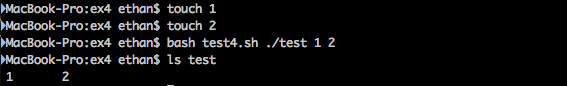
\includegraphics[width=0.7\textwidth]{3}
\end{image}

%%%%%%%%%%%%%%%%%%%%%%%%%%%%%%%%%%%%%%%%%%%%%%%%%%%%%%%%%
%   5
%%%%%%%%%%%%%%%%%%%%%%%%%%%%%%%%%%%%%%%%%%%%%%%%%%%%%%%%%
\begin{problem}
    打印给定目录下的某些文件,由第一个参数指出文件所在的目录,其余参数是要打印的文件名.
\end{problem}

\begin{answer}
    \lstinputlisting[language=sh,title=test5.sh]{../test5.sh}
\end{answer}

\begin{image}
    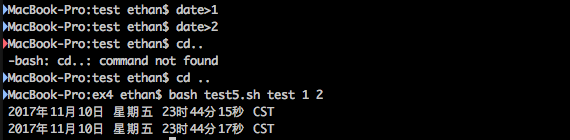
\includegraphics[width=0.7\textwidth]{4}
\end{image}

%%%%%%%%%%%%%%%%%%%%%%%%%%%%%%%%%%%%%%%%%%%%%%%%%%%%%%%%%
%   6
%%%%%%%%%%%%%%%%%%%%%%%%%%%%%%%%%%%%%%%%%%%%%%%%%%%%%%%%%
\begin{problem}
    利用 for 循环将当前目录下的.c 文件移到指定的目录下,并按文件大小排序,显示移动后指定目录的内容。
\end{problem}

\begin{answer}
    \lstinputlisting[language=sh,title=test6.sh]{../test6.sh}
\end{answer}

\begin{image}
    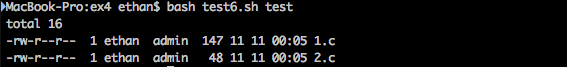
\includegraphics[width=0.7\textwidth]{5}
\end{image}
%%%%%%%%%%%%%%%%%%%%%%%%%%%%%%%%%%%%%%%%%%%%%%%%%%%%%%%%%
%   7
%%%%%%%%%%%%%%%%%%%%%%%%%%%%%%%%%%%%%%%%%%%%%%%%%%%%%%%%%
\begin{problem}
    编写一个 shell 脚本,求费波纳奇数列的前 10 项及总和.
\end{problem}

\begin{answer}
    \lstinputlisting[language=sh,title=test7.sh]{../test7.sh}
\end{answer}

\begin{image}
    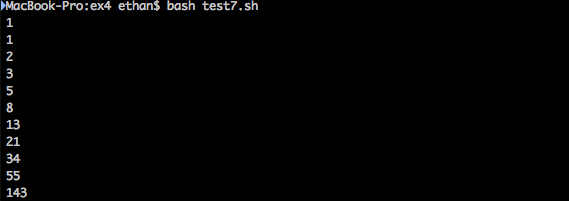
\includegraphics[width=0.7\textwidth]{6}
\end{image}


\section{实验体会}

这次实验我学会了使用shell脚本做一些简单的操作,由于是第一次写shell脚本,难免会感觉不熟悉。
比如有些关键字和语法结构与我们常用的C++不同,不过还是能体会shell脚本语言的简单高效,因为他
没有C++或者Java那么严谨,十分灵活。\\
\vfill

实验报告采用 \LaTeX 编写,代码托管至GitHub:\\
\url{https://github.com/Ethan-yt/JNU-Linux-exp}

\end{document}